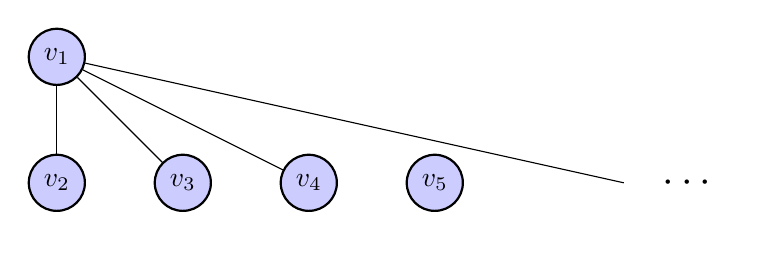
\begin{tikzpicture}
  [scale=.8,auto=left,every node/.style={circle,fill=blue!20,draw=black,thick}]
  \node (n1) at (0,2)  {$v_1$};
  \node (n2) at (0,0)  {$v_2$};
  \node (n3) at (2,0)  {$v_3$};
  \node (n4) at (4,0)  {$v_4$};
  \node (n5) at (6,0)  {$v_5$};


   \foreach \from/\to in {n1/n2,n1/n3, n1/n4}
      \draw (\from) -- (\to);
   
   \draw (n1) -- (9,0);

   \node[draw=none, fill=none, scale=1.5] at (10,0) {$\cdots$};
   
\end{tikzpicture}

